\documentclass[12pt,a4paper,twocolumn,twoside]{ujsikpb}
\usepackage{graphicx}
\usepackage{subcaption}
  \captionsetup[subfigure]{labelformat=simple}
  \renewcommand\thesubfigure{(\alph{subfigure})}
\usepackage{float}
\usepackage{placeins}
\usepackage{balance}

\setcounter{topnumber}{10}
\setcounter{dbltopnumber}{10}
\setcounter{bottomnumber}{10}
\setcounter{totalnumber}{10}
\renewcommand{\topfraction}{1.0}
\renewcommand{\bottomfraction}{1.0}
\renewcommand{\textfraction}{0.0}
\renewcommand{\floatpagefraction}{1.0}
\renewcommand{\dbltopfraction}{1.0}
\renewcommand{\dblfloatpagefraction}{1.0}

\begin{document}
\pagestyle{empty}

\thispagestyle{empty}
\articletype{研究論文}
\jtitle{医学生物学分野における高被引用論文の長期的影響と構造的特徴}
\etitle{Long-term impact and characteristics of highly cited papers in biomedical field}
\jauthor{天野晃$^{1*}$, 角田裕之$^{2}$, 孫媛$^{3}$, 西澤正己$^{3}$, 劉筱敏$^{4}$}
\eauthor{Kou AMANO, Hiroyuki TSUNODA, Yuan SUN, Masaki NISHIZAWA, Xiaomin LIU}
\affiliation{
$^{1}$ 鹿児島大学 \\
Kagoshima University \\
〒890-8980 鹿児島県鹿児島市郡元1丁目21-24 \\
$^{2}$ 東京大学 \\
University of Tokyo \\
$^{3}$ 国立情報学研究所 \\
National Institute of Informatics \\
〒101-8430 東京都千代田区一ツ橋2-1-2 \\
$^{4}$ 中国科学院文献情報中心 \\
$*$ EMail: k7085637@kadai.jp \\
}

\input{abstj.tex}
\eabstract{
This study aims to elucidate the long-term citation dynamics and structural characteristics of highly cited papers in the field of biomedical sciences. In conventional bibliometrics, short-term citation indicators such as the 3-year and 5-year impact factors have been predominantly used; however, long-term observation is essential for accurately capturing the true impact of scholarly articles. In this study, analysis was conducted from multiple perspectives, including citation lifespan, journal structure, and research topic structure, rather than relying solely on citation counts.
The dataset used was the PubMed Annual Baseline (2023), covering reference information from approximately 30 million papers published between 1946 and 2020. Based on this dataset, a “cumulative generation model” was constructed at five-year intervals, and the top 1\% of papers in terms of total citations within each cumulative generation were defined as “highly cited papers.” In addition, four groups were established to enable comparisons between highly cited papers and other papers.
At the individual paper level, the analysis revealed that even among highly cited papers, some of the most highly cited papers exhibited a long-lived pattern in which they did not reach obsolescence (citation decay) even several decades after publication. In contrast, among highly cited papers for which citation decline was observed, a lifespan structure was identified consisting of four years from publication to the citation peak and 12 years from publication to citation decay, which was consistent with existing models in the biological sciences.
At the journal level, it was shown that journals publishing many highly cited papers are not necessarily those with high impact factors. However, analysis using Kullback–Leibler divergence demonstrated that highly cited papers tend to exhibit a stronger concentration (preference) toward specific journals compared to other groups.
At the research topic level, entropy analysis based on MeSH descriptors revealed that highly cited papers are more concentrated in their research topics than other groups, and the topics of papers citing them are also similarly concentrated. At the same time, a divergence was observed between the topics of the cited papers and those of the citing papers, indicating that highly cited papers tend to be cited across different research fields.
}

\keywords{
高被引用論文;
被引用寿命;
オブソレッセンス \\
Keywords:
highly cited papers;
citation lifespan;
obsolescence
}


\maketitle

\section{背景と目的}
計量書誌学においては3年インパクトファクターや5年インパクトファクターなど\cite{Cla1}、特定の期間の（被）引用をもとにした指標が多く用いられる。
これは一面的には評価の公正性を考慮したものと考えられる。つまり、より古い論文ほど引用される機会は高くなり、この「論文の年齢」による効果を差し引くためである。
このような視点は雑誌の選定などにおいては重要なものである。一方で、長期に渡る引用の変化を把握することもまた重要である。第一に、前述の公正性における評価期間の設定の根拠となる。次に、短期的には捉えられない累積的な効果を捉えるには真に長期の観察が必要である。たとえば、引用という現象をより深く捉えるためには、単に（被）引用数に着目するだけでなく、引用関係とその変化などの構造的な面へのアプローチが望まれる。本研究では以上のような観点にたち、長期的な引用のダイナミクスを明らかにすることを試みる。
具体的には、1. 高被引用論文（定義は後述）の論文レベルでの長期的な被引用の構造、2. これらを掲載する雑誌の特徴（が見られるか）、3. これらの研究テーマ構造の長期的な変化（が見られるか）を、高被引用でない論文群と比較し分析する。


\section{関連研究}
高被引用論文や引用指標の研究は、近年も幅広い観点から進展している。Liら\cite{Li1}は2300万論文を対象に長期にわたる引用の特徴を分析しグループ構造を明らかにした。また、Yuら\cite{Yu1}は社会心理学分野のトップ被引用論文100本を対象とした構造解析により、主要な出版年・国際協力・ジャーナルの影響構造を明らかにし、被引用論文の研究ネットワーク構造に関する知見を提供している。 雑誌レベルに注目したものとして、Leydesdorff\cite{Ley1,Ley2,Ley3,Ley4}は雑誌間の関係マップを構築・調査した。天野ら\cite{Ama1,Ama2}は医学生物学雑誌の大規模クラスタリングを行い、分野間の引用関係を明らかにした。こうした研究は、高被引用論文あるいはハイインパクト誌がどのような条件下で生まれ、どのような影響経路を持つかをマクロ的な視点で捉える試みである。一方で、論文レベルの被引用に寄与する構造的因子の体系化も進んでおり、共同研究形態・出版戦略・研究資源配分などの多要因が被引用に影響する可能性が示唆されている。Hillら\cite{Hil1}は、研究者の研究テーマの転換戦略はむしろその後の影響を減少させる可能性を指摘した。Linら\cite{Lin1}は、被引用論文の全文データを用いて、引用の位置・文脈・引用者との類似性が経時的に変化する現象を観察し、単なる引用数では捉えきれない引用の役割の変容を指摘している。Koushaら\cite{Ko1}は、情報科学分野の論文に対し、抄録の「読みやすさ」と論文の「質」が、被引用数にどのように影響するかを調査した。以上紹介した研究は主として被引用性にかかるさまざまな属性の特徴を明らかにするものであるが、高被引用論文に共通する長期的構造特性そのものを多層的に捉える研究は限定的である。本研究は、引用寿命・雑誌構造・テーマ構造などの要素を統合的に分析することで既存研究とは異なる視点を提供する。


\section{マテリアル}
本研究では、長期的な引用ダイナミクスを把握するため、単年ごとの分析ではなく、ある程度の時間幅（世代）を考慮した引用の累積的効果を反映するモデルを構成する。また、長期間に渡り引用関係を捕捉できるデータとしてPubMedを用いる。さらにPubMedには各論文に統制語（MeSH）が付与されているため、高被引用論文に付与されるMeSHディスクリプターを計量的に分析することにより、研究テーマに関するマクロな構造を見出せると期待される。

\subsection{データ}
本研究では、FTP版のPubMed annual baseline (2023)（以降、PubMedとする）\cite{PM1}を利用する。本研究の対象は1946年から2020年までに出版された論文約3000万件に記載されるレファレンス情報である。
したがって、対象となる論文には1946年よりも古い出版のものも含む。


\subsection{累積世代モデル}
本研究では、累積的な変化を捉えるために累積的な世代を構成する。まず、1946-2020の出版年をオーバーラップなしの5年ごとの区切りとした15層に分け、これらを累積的に構成する。これを累積世代モデルと称する。構成前の各層の登録論文数、うち参考文献を持つ論文数、引用された論文数、引用数、雑誌数を図\ref{fig:gr2}に示す。雑誌数以外は指数関数的な増加を示している。

\begin{figure}[h]
\begin{center}
  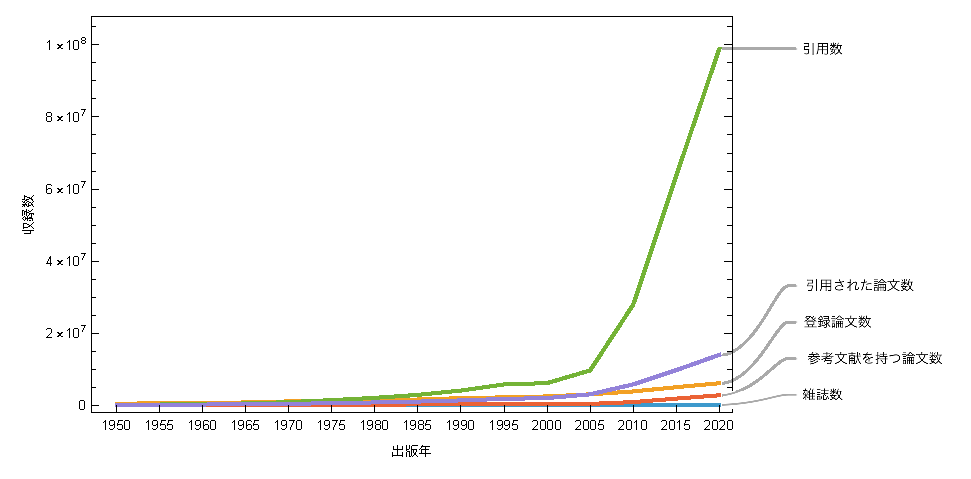
\includegraphics[width=75mm]{Main-manuscript_V4_gr2.eps}
  \caption{5年ごとの収録論文数}
  \label{fig:gr2}
\end{center}
\end{figure}


\subsection{高被引用論文・高被引用論文掲載誌・高被引用テーマ}
本研究では、各累積世代において被引用数全体の1\%を構成する被引用数上位の論文群を「高被引用論文」と定義する。これらを掲載した雑誌を「高被引用論文掲載誌」、高被引用論文に付与されるMeSHディスクリプターを「高被引用テーマ」と定義する。さらに高被引用論文を引用する論文群を考え、これらの論文に付与されるMeSHディスクリプターを「高被引用論文引用テーマ」とする。
また、論文に付与されるMeSHディスクリプター一般を「研究テーマ」、論文が引用関係にある場合、引用される論文に付与されるMeSHディスクリプターを「被引用テーマ」、引用する論文に付与されるMeSHディスクリプターを「引用テーマ」とする。以上の定義をまとめたものを表\ref{tab:def}に示す。

\begin{table}[h]
\begin{center}
\caption{本研究での用語定義} \label{tab:def}
{\small
\begin{tabular}{lp{32mm}}
  用語 & 定義 \\
  \hline 
  高被引用論文 & 被引用数全体の1\%を構成する被引用数上位論文 \\
  高被引用論文掲載誌 & 高被引用論文を出版した雑誌 \\
  高被引用テーマ & 高被引用論文に付与されるMeSHディスクリプター \\
  高被引用論文引用テーマ & 高被引用論文を引用する論文に付与されるMeSHディスクリプター \\
  研究テーマ & 論文に付与されるMeSHディスクリプター \\
  引用テーマ & 論文を引用する論文に付与されるMeSHディスクリプター \\
  被引用テーマ & 論文に引用される論文に付与されるMeSHディスクリプター \\
\end{tabular}
}
\end{center}
\end{table}


\subsection{比較グループ}
のちに高被引用論文とその他の論文とを比較するため、各累積世代で高被引用論文を含め全4グループを構成する。論文を被引用数の大きい順に並べ、被引用数の累積和に基づいて総被引用数を100分した際の、累積被引用数の0-1%区間に相当する論文群をG1すなわち高被引用論文、25-26%区間にある論文群をG2、50-51i%区間にある論文群をG3、75-76%区間にある論文群をG4とする。


\section{高被引用論文}
\subsection{高被引用論文の出現}
\begin{figure*}[t]
\centering

\begin{subfigure}{0.32\textwidth}
  \centering
  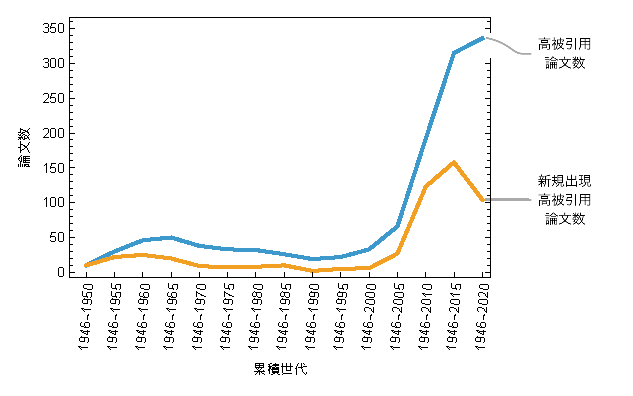
\includegraphics[width=\linewidth]{gr3.eps}
  \caption{高被引用論文および新規出現高被引用論文の出現数}
  \label{fig:gr3}
\end{subfigure}
\hfill
\begin{subfigure}{0.32\textwidth}
  \centering
  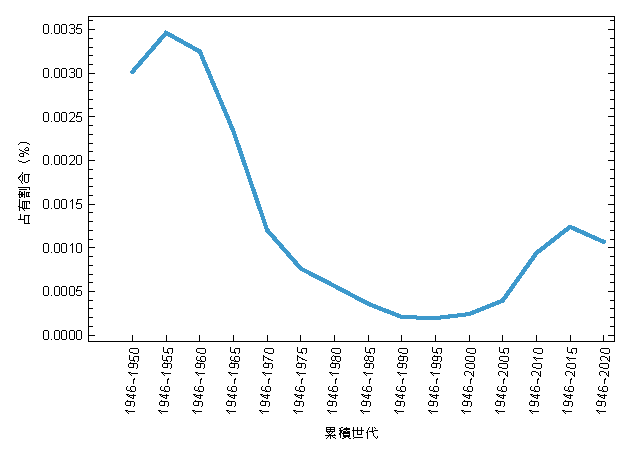
\includegraphics[width=\linewidth]{gr4.eps}
  \caption{高被引用論文の全論文に占める割合（\%）}
  \label{fig:gr4}
\end{subfigure}
\hfill
\begin{subfigure}{0.32\textwidth}
  \centering
  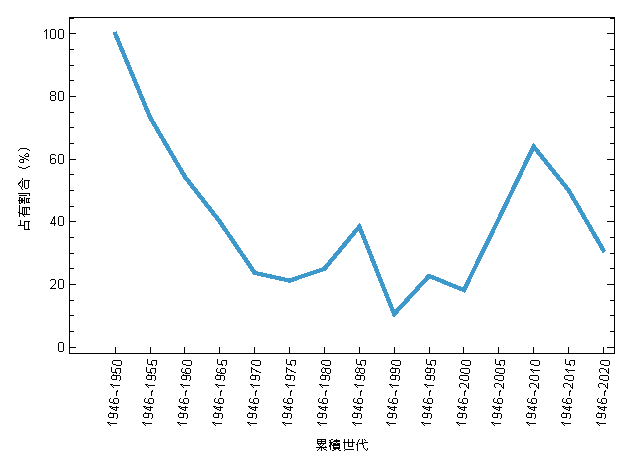
\includegraphics[width=\linewidth]{gr5.eps}
  \caption{新規出現高被引用論文の高被引用論文に占める割合（\%）}
  \label{fig:gr5}
\end{subfigure}

\caption{高被引用論文群の統計}
\label{fig:array1all}
\end{figure*}

高被引用論文の出現数を図\ref{fig:gr3}に示す。高被引用論文数および新規出現高被引用論文数は1946-2010年の累積世代以降に急増しているが、これは近年の収録論文数の急増を受けたものであると思われる。高被引用論文の影響性を確認するため、高被引用論文の全論文に占める割合を図\ref{fig:gr4}に示す。被引用数の1\%を最大でも全体の0.0035\%の論文が構成しており、被引用の集中度の高さが見て取れる。経時変化に一定の傾向はなく緩やかな変動が見られる。高被引用論文の入れ替わりを確認するため、新規高被引用論文の高被引用論文に占める割合を図5に示す。経時変化に一定の傾向は観察されず、概ね10\%から60\%のメンバーの入れ替わりが見られる。


\subsection{高被引用論文の変遷}
ここでは高被引用論文の変遷をさらに詳しく見るために論文順位の変動を観察する。
Kendallの順位相関を使いた比較を年ごとに行えば、相関係数が高いほど順位変動が少ない、すなわち安定していると見做せる。
対象はすべての累積世代の高被引用論文（536論文）とし、1947-2020年までの各年につき、前年と比較した際の相関係数を算出した。
図\ref{fig:gr101}に各年の相関係数を示す。
値は0.8-0.95の間を推移し、経過年による傾向は見られない。
さらに、累積的な被引用の効果がどのように現れるかを確認するため、出版後n年までの累積被引用数を用いた場合と比較した。
完全な累積型との相関係数の差を図\ref{fig:gr102}に示す。
これによれば、影響年を制限するほど相関係数が高くなる、すなわち順位が安定する傾向があり、被引用における累積的な影響は順位を変動させる要因となる可能性が高い。

各累積世代の最多被引用論文とその被引用数を表\ref{tab:mostcitedA}に示す。最多被引用論文は累積世代が進んでも引き続き引用され続ける傾向があり、数十年をかけてインパクトを上昇させている。このため最多被引用論文の交代は少ない。これらはいずれも論文タイトルおよび高被引用テーマを見る限りタンパク質に関するものである。

\begin{figure}[h]
\begin{center}
  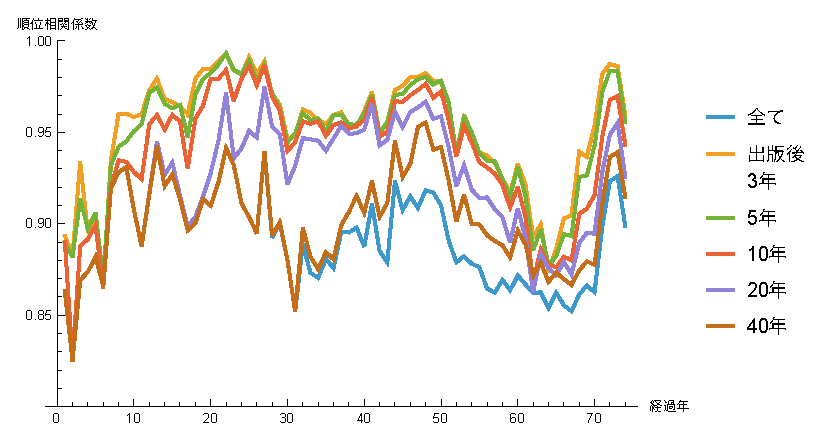
\includegraphics[width=76mm]{kendallall.eps}
  \caption{順位相関係数 \newline すべての累積を用いた順相関係数と出版後n 年まで
の累積を用いた順位相関係数。}
  \label{fig:gr101}
\end{center}
\end{figure}

\begin{figure}[h]
\begin{center}
  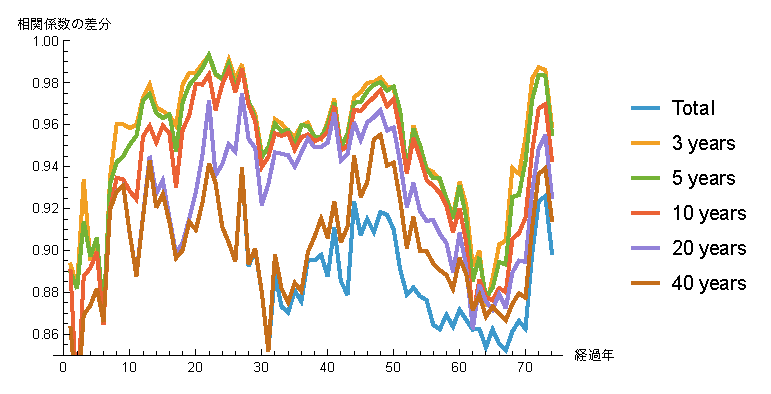
\includegraphics[width=76mm]{kendalldiff.eps}
  \caption{順位相関係数の差}
  \label{fig:gr102}
\end{center}
\end{figure}

%\subsection{最多被引用論文の変遷}
\input{tabarray-hctitlesA.utf8.tex}

\subsection{高被引用論文のオブソレッセンス}
ここでは、高被引用論文の影響が長期的にどのように変化するかを分析するため、オブソレッセンスに注目し、寿命構造を観察する。
まず、オブソレッセンス状態を判定するために、Sun\cite{SUn1}らの提案する Obsolescence vector を導入する。
Obsolescence vector はGini係数の派生であり$O(Gs,A^-)$で表されるが、本研究では$O(Gs,A^-,A^+)$を用いる。$Gs$は、Gini係数に相当し、値が小さいほど相対的に引用が早期に偏っていることを示し、$|A^-|$、$|A^+|$はローレンツ曲線による面積の一部であり、その値はそれぞれ被引用の減少および増加の変化の速さを示す（図\ref{fig:obsvec}）。

さらに、Paroloら\cite{Par1}、Wangら\cite{Wan1}のモデルを勘案し、この指標を用いて高被引用論文を次の5クラス（FP/SB/Nm/G/O）に分類する。
うち、クラスNmについては、のちの分析のためさらにサブクラスNoを設ける。
\begin{itemize}
\item FP; Flash in the pan：Sunらは Flash in the pan の基準として、$Gs=-0.600$、$A^- = -0.300$ を示している。本研究ではこの値を参照し、$Gs < -0.600$ かつ $A^- < -0.300$ の値を持つ論文を Flash in the pan とする。
\item SB; Sleeping beauty：Sunらは $A^+$ を用いた Sleeping beauty の基準を示していないが、本研究では Flash in the pan と対照的な条件として $Gs > 0.600$ かつ $A^+ > 0.300$ の値を持つ論文を Sleeping beauty とする。
\item Nm; 成熟論文：Flash in the pan にも Sleeping beauty にも含まれない標準的かつある程度引用を得た論文の条件として、$-0.600 \leq Gs \leq 0.600$ かつ $A^- < 0$ かつ $A^+ > 0$ かつ $|A^-| > |A^+|$ を設定し、これに当てはまる論文を成熟論文とする。
\item No; 成熟論文のうちオブソレッセンスが確認されるもの：成熟論文のうちオブソレッセンスの傾向が強いものとして $A^- < -0.1$ となる論文集合を設定する。
\item G; 成長論文：被引用が成長段階にある論文として、$-0.600 \leq Gs \leq 0.600$ かつ $A^- = 0$ を設定する。
\item O; その他：以上の条件に含まれないものとして特殊な被引用形状のもの（本研究で前提としているモデルである対数正規分布に合致しないリバイバル論文等）が考えられる。
\end{itemize}

表\ref{tab:obsindex}に各クラスの指標値（中央値）を示す。高被引用論文ではクラスG（成長論文）が最も多く、次にクラスNm、クラスOと続き、クラスFPとクラスSBは同程度に出現している。なお、クラスFP（Flash in the pan）の年齢が高いのは、このクラスに分類されるには、早期の高い被引用だけでなくその後の十分な低い被引用期間も要することによる。
表\ref{tab:mcpobsindex}に最多被引用論文の指標値を示す。最多被引用論文の各指標値の範囲は広く、必ずしも特定のクラスから出現するわけではないことを示唆している。なお、うち2本はクラスOに分類されているが、被引用曲線を確認したところ明確な多峰性が見られ、リバイバル論文であることが明らかであった。

\begin{figure}[h]
\begin{center}
  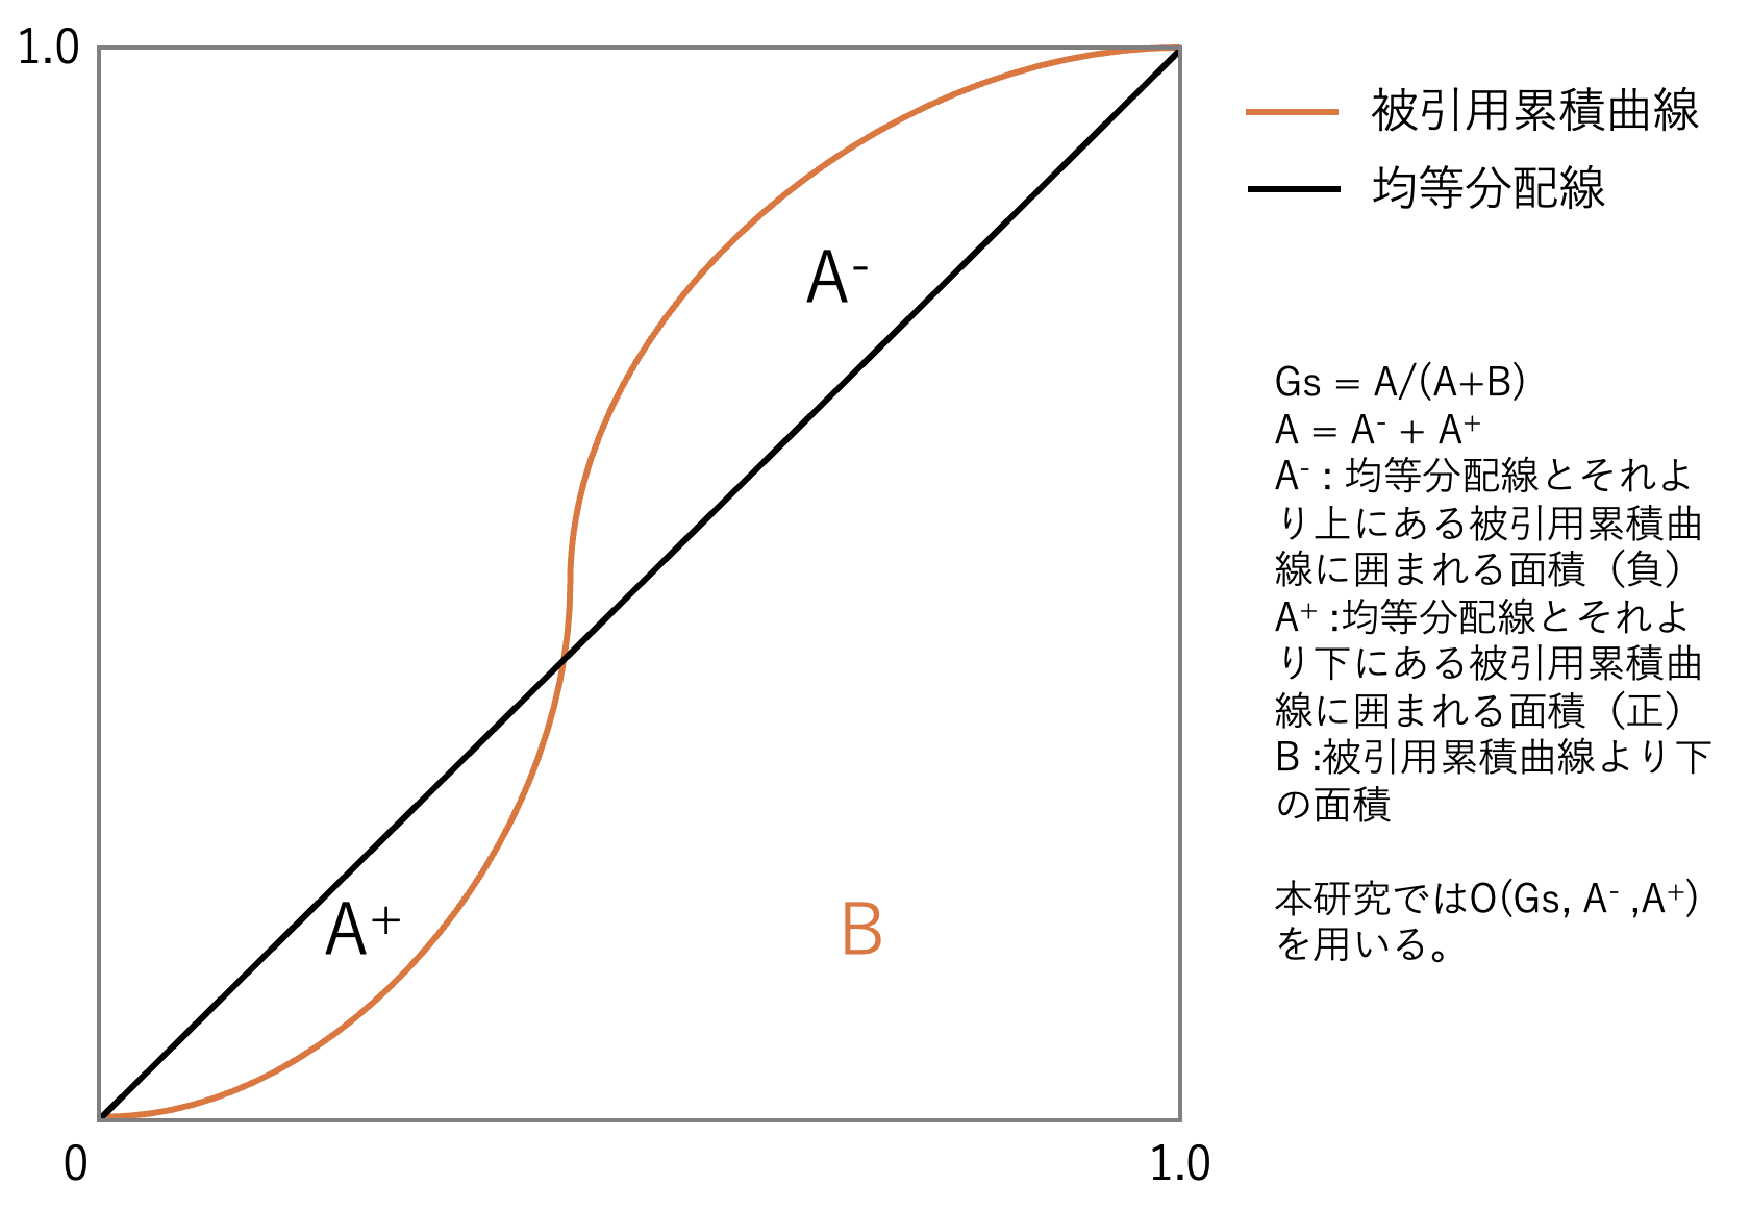
\includegraphics[width=76mm]{obsvec.eps}
  \caption{Obsolescence vector}
  \label{fig:obsvec}
\end{center}
\end{figure}

\begin{table*}
\begin{center}
\caption{高被引用論文のオブソレッセンスにかかる各指標値（中央値）} \label{tab:obsindex}
\begin{tabular}{lllllr}
クラス & $A^-$ & $A^+$ & Gs & 年齢 & メンバー数(\%)\\
\hline
FP & -0.346 & 0. & -0.691 & 70. & 29(5) \\
Nm & -0.116 & 0.005 & -0.323 & 44. & 150(28) \\
No & -0.192 & 0.004 & -0.374 & 49.5 & 114(21) \\
SB & 0. & 0.336 & 0.671 & 35. & 30(6) \\
O & 0. & 0.147 & 0.295 & 17. & 327(61) \\
\end{tabular}
\end{center}
\end{table*}


\section{高被引用論文掲載誌}
引用の構造は出版媒体（雑誌）という制度的単位とも深く関係している。
そこで本章では論文レベルの特性が雑誌という切り口ではどのように現れるかを見るため、高被引用論文を掲載する雑誌（高被引用論文掲載誌）に注目する。

\subsection{高被引用論文掲載誌の出現}
\input{journalwithhcp-no-syutugen.tex}
\begin{figure*}[t]
\centering

\begin{subfigure}{0.32\textwidth}
  \centering
  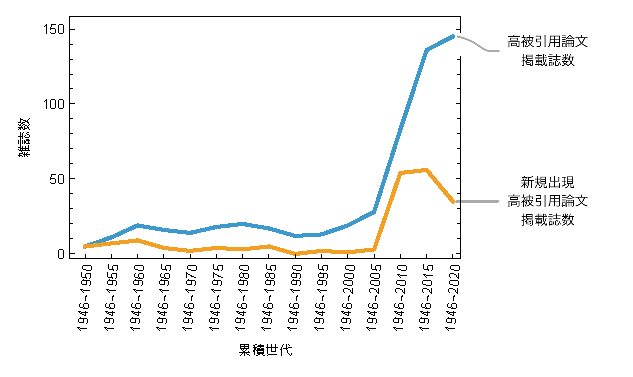
\includegraphics[width=\linewidth]{gr9.eps}
  \caption{高被引用論文掲載誌および新規出現高被引用論文掲載誌の出現数}
  \label{fig:gr9}
\end{subfigure}
\hfill
\begin{subfigure}{0.32\textwidth}
  \centering
  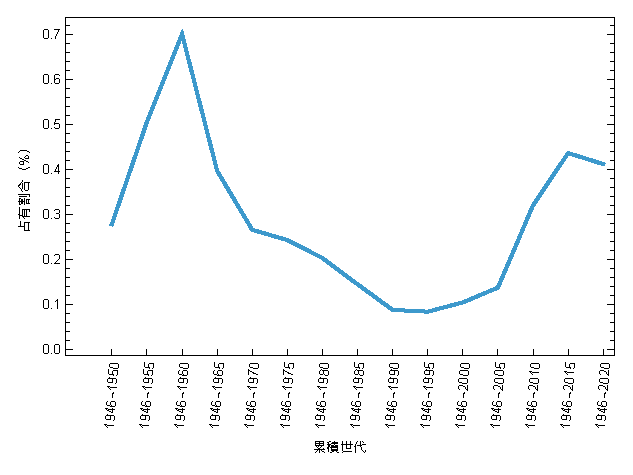
\includegraphics[width=\linewidth]{gr10.eps}
  \caption{高被引用論文掲載誌の全雑誌に占める割合（\%）}
  \label{fig:gr10}
\end{subfigure}
\hfill
\begin{subfigure}{0.32\textwidth}
  \centering
  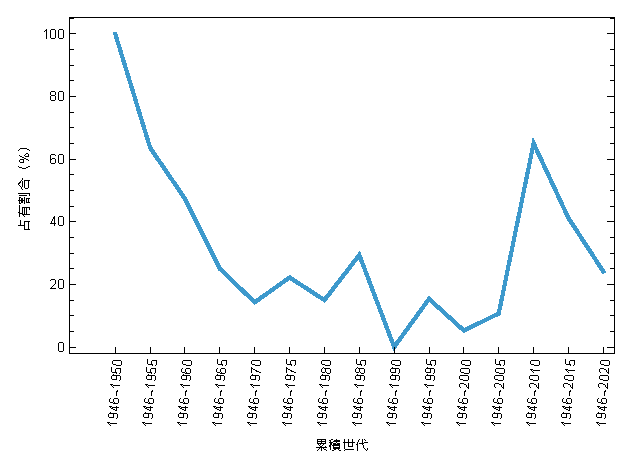
\includegraphics[width=\linewidth]{gr11.eps}
  \caption{新規出現高被引用論文掲載誌の高被引用論文掲載誌に占める割合（\%）}
  \label{fig:gr11}
\end{subfigure}

\caption{高被引用論文掲載誌の統計}
\label{fig:array2all}
\end{figure*}


\subsection{高被引用論文掲載誌の変遷}
ここでは高被引用論文掲載誌の変化を高被引用でないグループのそれと比較する。G1-G4の当該論文の掲載数上位の雑誌一覧を表\ref{tab:G1topj}-\ref{tab:G4topj}に示す。各誌のインパクトファクターとその発表年についてはJournal Citation Reports  (JCR）[JCR1]から求めた。JCRではインパクトファクターの公開が1997からであるため、1946-2000年の累積世代以降についてのみ、累積世代の最終年のインパクトファクターを求めた。ここから、高被引用論文を持つ雑誌は必ずしもインパクトファクターが高い雑誌ではないことがわかる。一方、雑誌の構成においてはグループ間に特別な差異を認めらない。そこで、各グループでどの程度の雑誌の嗜好があるかを確認するため、全てのグループを合成した集団と各グループとの間でKullback-Leibler divergence（KLD）を求めたものを図14に示す。図14からは、高被引用論文は他のグループに比べ雑誌の嗜好が強いことが明らかになった。

\begin{figure}[h]
\begin{center}
  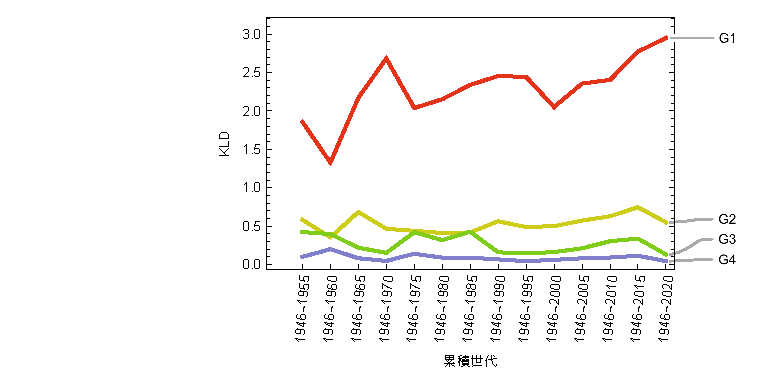
\includegraphics[width=75mm]{Main-manuscript_V4_gr12.eps}
  \caption{各グループの雑誌の構成に関するKLD}
  \label{fig:gr12}
\end{center}
\end{figure}

\begin{table*}[h]
\begin{center}
\caption{高被引用論文掲載誌のうち最大の論文数を持つもの} \label{tab:G1topj}
{\tiny
\[\begin{array}{ccccc}
 {累積世代} & 
\begin{array}{p{20mm}}
 {雑誌タイトル} \\
\end{array}
 & 
\begin{array}{p{14mm}}
 {当該誌の高被引用論文数} \\
\end{array}
 & 
\begin{array}{p{14mm}}
 {当該誌の高被引用論文が当該累積世代の高被引用論文全体に占める割合（\%）} \\
\end{array}
 & 
\begin{array}{c}
 {IF/発表年} \\
\end{array}
 \\
 {1946-1950} & 
\begin{array}{p{20mm}}
 {The Journal of clinical investigation} \\
 {The Biochemical journal} \\
\end{array}
 & 
\begin{array}{c}
 3 \\
 3 \\
\end{array}
 & 30 & 
\begin{array}{c}
 {12.015/2000}; {15.053/2005}; {14.152/2010}; {12.575/2015}; {14.808/2020} \\
 {4.28/2000}; {4.224/2005}; {5.016/2010}; {3.562/2015}; {3.857/2020} \\
\end{array}
 \\
 {1946-1955} & 
\begin{array}{p{20mm}}
 {上記と同じ} \\
\end{array}
 & 
\begin{array}{c}
 13 \\
\end{array}
 & 43 & 
\begin{array}{c}
 {上記と同じ} \\
\end{array}
 \\
 {1946-1960} & 
\begin{array}{p{20mm}}
 {上記と同じ} \\
\end{array}
 & 
\begin{array}{c}
 11 \\
\end{array}
 & 24 & 
\begin{array}{c}
 {上記と同じ} \\
\end{array}
 \\
 {1946-1965} & 
\begin{array}{p{20mm}}
 {上記と同じ} \\
\end{array}
 & 
\begin{array}{c}
 13 \\
\end{array}
 & 26 & 
\begin{array}{c}
 {上記と同じ} \\
\end{array}
 \\
 {1946-1970} & 
\begin{array}{p{20mm}}
 {上記と同じ} \\
\end{array}
 & 
\begin{array}{c}
 9 \\
\end{array}
 & 24 & 
\begin{array}{c}
 {上記と同じ} \\
\end{array}
 \\
 {1946-1975} & 
\begin{array}{p{20mm}}
 {The Journal of biological chemistry} \\
\end{array}
 & 
\begin{array}{c}
 7 \\
\end{array}
 & 21 & 
\begin{array}{c}
 {7.368/2000}; {5.854/2005}; {5.328/2010}; {4.258/2015}; {5.157/2020} \\
\end{array}
 \\
 {1946-1980} & 
\begin{array}{p{20mm}}
 {上記と同じ} \\
\end{array}
 & 
\begin{array}{c}
 7 \\
\end{array}
 & 22 & 
\begin{array}{c}
 {上記と同じ} \\
\end{array}
 \\
 {1946-1985} & 
\begin{array}{p{20mm}}
 {上記と同じ} \\
\end{array}
 & 
\begin{array}{c}
 5 \\
\end{array}
 & 19 & 
\begin{array}{c}
 {上記と同じ} \\
\end{array}
 \\
 {1946-1990} & 
\begin{array}{p{20mm}}
 {上記と同じ} \\
\end{array}
 & 
\begin{array}{c}
 4 \\
\end{array}
 & 21 & 
\begin{array}{c}
 {上記と同じ} \\
\end{array}
 \\
 {1946-1995} & 
\begin{array}{p{20mm}}
 {上記と同じ} \\
\end{array}
 & 
\begin{array}{c}
 4 \\
\end{array}
 & 18 & 
\begin{array}{c}
 {上記と同じ} \\
\end{array}
 \\
 {1946-2000} & 
\begin{array}{p{20mm}}
 {Journal of molecular biology} \\
 {Proceedings of the National Academy of Sciences of the United States of America} \\
\end{array}
 & 
\begin{array}{c}
 4 \\
 4 \\
\end{array}
 & 12 & 
\begin{array}{c}
 {5.388/2000}; {5.229/2005}; {4.008/2010}; {4.517/2015}; {5.469/2020} \\
 {10.789/2000}; {10.231/2005}; {9.771/2010}; {9.423/2015}; {11.205/2020} \\
\end{array}
 \\
 {1946-2005} & 
\begin{array}{p{20mm}}
 {Proceedings of the National Academy of Sciences of the United States of America} \\
\end{array}
 & 
\begin{array}{c}
 8 \\
\end{array}
 & 12 & 
\begin{array}{c}
 {10.789/2000}; {10.231/2005}; {9.771/2010}; {9.423/2015}; {11.205/2020} \\
\end{array}
 \\
 {1946-2010} & 
\begin{array}{p{20mm}}
 {Proceedings of the National Academy of Sciences of the United States of America} \\
 {Nature} \\
\end{array}
 & 
\begin{array}{c}
 14 \\
 14 \\
\end{array}
 & 7 & 
\begin{array}{c}
 {10.789/2000}; {10.231/2005}; {9.771/2010}; {9.423/2015}; {11.205/2020} \\
 {25.814/2000}; {29.273/2005}; {36.104/2010}; {38.138/2015}; {49.962/2020} \\
\end{array}
 \\
 {1946-2015} & 
\begin{array}{p{20mm}}
 {Nature} \\
\end{array}
 & 
\begin{array}{c}
 20 \\
\end{array}
 & 6 & 
\begin{array}{c}
 {25.814/2000}; {29.273/2005}; {36.104/2010}; {38.138/2015}; {49.962/2020} \\
\end{array}
 \\
 {1946-2020} & 
\begin{array}{p{20mm}}
 {Bioinformatics (Oxford, England)} \\
\end{array}
 & 
\begin{array}{c}
 17 \\
\end{array}
 & 5 & 
\begin{array}{c}
 {3.409/2000}; {6.019/2005}; {4.877/2010}; {5.766/2015}; {6.937/2020} \\
\end{array}
 \\
\end{array}\]
}
\end{center}
\end{table*}

\begin{table*}[h]
\begin{center}
\caption{G2論文掲載誌のうち最大の論文数を持つもの} \label{tab:G2topj}
{\tiny
\[\begin{array}{cp{20mm}ccc}
 {累積世代} & {雑誌タイトル} & {当該誌のG2論文数} & {\begin{array}{p{14mm}}当該誌のG2論文が当該累積世代のG2論文全体に占める割合（\%）\end{array}} & {IF / 発表年} \\
\hline
 {1946-1950} & {Journal of bacteriology} & 34 & 45 & {3.506/2000; 4.167/2005; 3.726/2010; 3.198/2015; 3.49/2020} \\
 {1946-1955} & {The Biochemical journal} & 20 & 7 & {4.28/2000; 4.224/2005; 5.016/2010; 3.562/2015; 3.857/2020} \\
 {1946-1960} & {上記と同じ} & 64 & 10 & {上記と同じ} \\
 {1946-1965} & {上記と同じ} & 62 & 7 & {上記と同じ} \\
 {1946-1970} & {The Journal of biological chemistry} & 90 & 6 & {7.368/2000; 5.854/2005; 5.328/2010; 4.258/2015; 5.157/2020} \\
 {1946-1975} & {The Journal of physiology} & 98 & 5 & {4.455/2000; 4.272/2005; 5.139/2010; 4.731/2015; 5.182/2020} \\
 {1946-1980} & {The Journal of biological chemistry} & 150 & 5 & {7.368/2000; 5.854/2005; 5.328/2010; 4.258/2015; 5.157/2020} \\
 {1946-1985} & {Proceedings of the National Academy of Sciences of the United States of America} & 214 & 6 & {10.789/2000; 10.231/2005; 9.771/2010; 9.423/2015; 11.205/2020} \\
 {1946-1990} & {上記と同じ} & 316 & 7 & {上記と同じ} \\
 {1946-1995} & {上記と同じ} & 410 & 7 & {上記と同じ} \\
 {1946-2000} & {上記と同じ} & 490 & 7 & {上記と同じ} \\
 {1946-2005} & {上記と同じ} & 715 & 7 & {上記と同じ} \\
 {1946-2010} & {上記と同じ} & 947 & 6 & {上記と同じ} \\
 {1946-2015} & {上記と同じ} & 882 & 5 & {上記と同じ} \\
 {1946-2020} & {Proceedings of the National Academy of Sciences of the United States of America} & 810 & 3 & {10.789/2000; 10.231/2005; 9.771/2010; 9.423/2015; 11.205/2020} \\
\end{array}\]
}
\end{center}
\end{table*}

\begin{table*}[h]
\begin{center}
\caption{G3論文掲載誌のうち最大の論文数を持つもの}
{\tiny
\[\begin{array}{cp{20mm}ccc}
 {累積世代} & {雑誌タイトル} & {当該誌のG3論文数} & {\begin{array}{p{14mm}}当該誌のG3論文が当該累積世代のG3論文全体に占める割合（\%）\end{array}} & {IF / 発表年} \\
 {1946-1950} & {The Biochemical journal} & 41 & 24 & {4.28/2000 4.224/2005 5.016/2010 3.562/2015 3.857/2020} \\
 {1946-1955} & {The Journal of biological chemistry} & 21 & 4 & {7.368/2000 5.854/2005 5.328/2010 4.258/2015 5.157/2020} \\
 {1946-1960} & {Proceedings of the Society for Experimental Biology and Medicine. Society for Experimental Biology and Medicine
(New York, N.Y.)} & 71 & 5 & {3.415/2000 -/2005 -/2010 -/2015 -/2020} \\
 {1946-1965} & {The Journal of biological chemistry} & 72 & 3 & {7.368/2000 5.854/2005 5.328/2010 4.258/2015 5.157/2020} \\
 {1946-1970} & {上記と同じ} & 116 & 3 & {上記と同じ} \\
 {1946-1975} & {上記と同じ} & 205 & 4 & {上記と同じ} \\
 {1946-1980} & {上記と同じ} & 267 & 4 & {上記と同じ} \\
 {1946-1985} & {Proceedings of the National Academy of Sciences of the United States of America} & 388 & 4 & {10.789/2000 10.231/2005
9.771/2010 9.423/2015 11.205/2020} \\
 {1946-1990} & {The Journal of biological chemistry} & 440 & 4 & {7.368/2000 5.854/2005 5.328/2010 4.258/2015 5.157/2020} \\
 {1946-1995} & {上記と同じ} & 782 & 5 & {上記と同じ} \\
 {1946-2000} & {上記と同じ} & 897 & 5 & {上記と同じ} \\
 {1946-2005} & {上記と同じ} & 1419 & 5 & {上記と同じ} \\
 {1946-2010} & {上記と同じ} & 1681 & 4 & {上記と同じ} \\
 {1946-2015} & {上記と同じ} & 1976 & 4 & {上記と同じ} \\
 {1946-2020} & {上記と同じ} & 1678 & 2 & {上記と同じ} \\
\end{array}\]
}
\end{center}
\end{table*}

\begin{table*}[h]
\begin{center}
\caption{G4論文掲載誌のうち最大の論文数を持つもの} \label{tab:G4topj}
{\tiny
\[\begin{array}{cp{20mm}ccc}
 {累積世代} & {雑誌タイトル} & {当該誌のG4論文数} & {\begin{array}{p{14mm}}当該誌のG4論文が当該累積世代のG4論文全体に占める割合（\%）\end{array}} & {IF / 発表年} \\
\hline
 {1946-1950} & {Annals of surgery} & 34 & 10 & {5.987/2000; 6.328/2005; 7.474/2010; 8.569/2015; 12.969/2020} \\
 {1946-1955} & {上記と同じ} & 105 & 6 & {上記と同じ} \\
 {1946-1960} & {The Biochemical journal} & 240 & 10 & {4.28/2000; 4.224/2005; 5.016/2010; 3.562/2015; 3.857/2020} \\
 {1946-1965} & {Nature} & 121 & 3 & {25.814/2000; 29.273/2005; 36.104/2010; 38.138/2015; 49.962/2020} \\
 {1946-1970} & {British medical journal} & 185 & 2 & {5.331/2000; 9.052/2005; 13.471/2010; -/2015 -/2020} \\
 {1946-1975} & {Biochimica et biophysica acta} & 290 & 3 & {-/2000; -/2005; -/2010; -/2015; -/2020} \\
 {1946-1980} & {上記と同じ} & 489 & 3 & {上記と同じ} \\
 {1946-1985} & {The Journal of biological chemistry} & 627 & 3 & {7.368/2000; 5.854/2005; 5.328/2010; 4.258/2015; 5.157/2020} \\
 {1946-1990} & {Biochimica et biophysica acta} & 842 & 3 & {-/2000; -/2005; -/2010; -/2015; -/2020} \\
 {1946-1995} & {The Journal of biological chemistry} & 1142 & 3 & {7.368/2000; 5.854/2005; 5.328/2010; 4.258/2015; 5.157/2020} \\
 {1946-2000} & {上記と同じ} & 1770 & 4 & {上記と同じ} \\
 {1946-2005} & {上記と同じ} & 1375 & 2 & {上記と同じ} \\
 {1946-2010} & {上記と同じ} & 2093 & 2 & {上記と同じ} \\
 {1946-2015} & {PloS one} & 3117 & 2 & {-/2000; -/2005; 4.411/2010; 3.057/2015; 3.24/2020} \\
 {1946-2020} & {上記と同じ} & 3560 & 2 & {上記と同じ} \\
\end{array}\]
}
\end{center}
\end{table*}


\section{高被引用テーマ}
本章ではさらに視点を変え、研究内容に関する構造的な差を明らかにするため論文のテーマに着目する。

\subsection{高被引用テーマの出現}
\begin{figure*}[h]
\centering

\begin{subfigure}{0.32\textwidth}
  \centering
  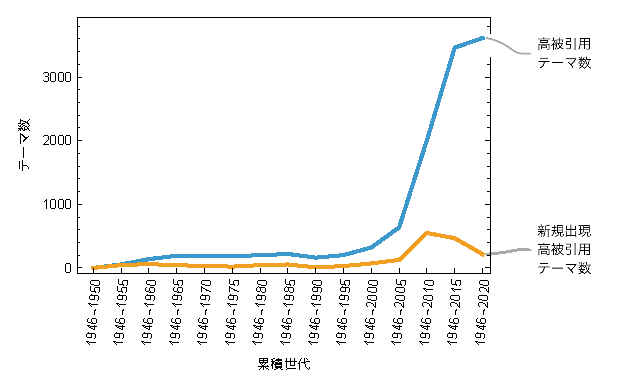
\includegraphics[width=\linewidth]{gr13.eps}
  \caption{高被引用テーマおよび新規出現高被引用テーマの出現数}
  \label{fig:gr13}
\end{subfigure}
\hfill
\begin{subfigure}{0.32\textwidth}
  \centering
  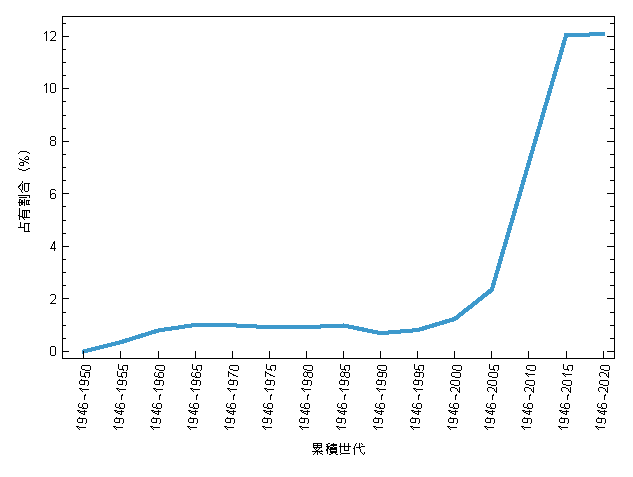
\includegraphics[width=\linewidth]{gradd1.eps}
  \caption{高被引用テーマの全出現テーマに占める割合（\%）}
  \label{fig:gradd1}
\end{subfigure}
\hfill
\begin{subfigure}{0.32\textwidth}
  \centering
  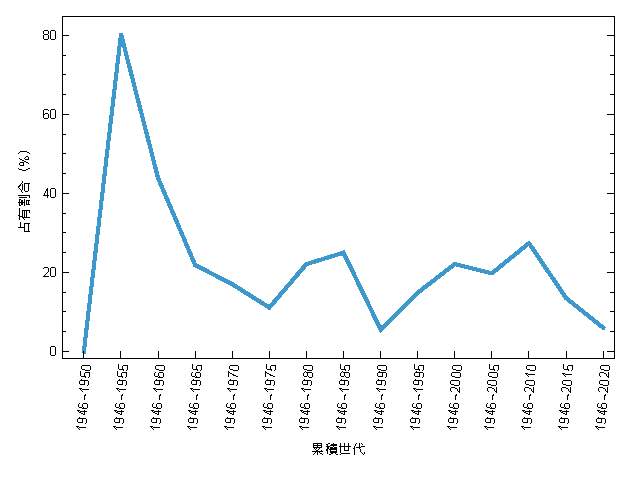
\includegraphics[width=\linewidth]{gr14.eps}
  \caption{新規出現高被引用テーマの高被引用テーマ全体に占める割合（\%）}
  \label{fig:gr14}
\end{subfigure}

\caption{高被引用論文掲載誌の統計}
\label{fig:array2all}
\end{figure*}

高被引用テーマのユニーク出現数を図\ref{fig:gr13}に示す。2023年MeSHディスクリプターの総数はおよそ30000であるが、各累積世代における高被引用テーマの出現数は最大でも3000を超える程度であり高被引用テーマには集中が見られる。高被引用テーマの入れ替わりを確認するため、新規出現高被引用テーマの高被引用テーマ全体に占める割合を図\ref{fig:gr14}に示す。経時的に一定の傾向は観察されず、数\%から十数\%の範囲での入れ替わりが観察される。なお、1946-1955年の累積世代に高い値が見られる理由は、前累積世代ではMeSHディスクリプターの付与がほとんどなかったためである。


\subsection{高被引用テーマの変遷}
ここでは高被引用テーマの変化を、高被引用でない論文のそれと比較する。
各累積世代、各グループごとの最頻出被引用テーマと引用テーマを表\ref{tab:topmesh}に示す。これらのうちG1の被引用テーマ（高被引用テーマ）にのみにバラエティが確認される。
次に、各累積世代の被引用テーマと引用テーマの多様性を見るために各グループのエントロピーの変化を観察した。被引用テーマ、引用テーマ、被引用テーマと引用テーマ対の出現数のエントロピーを、それぞれ図\ref{fig:arr2}に示す。計数の方法は、被引用テーマと引用テーマについては、それぞれ論文ごとの分数カウントを採用する。被引用テーマ対引用テーマのペアについては、ひとつの参照ごとに被引用テーマと引用テーマの2部グラフを構成し、エッジの重みの合計が1となる分数カウントを採用する。図\ref{fig:arr2}からは高被引用論文のみがエントロピーが低く、その他のグループ間ではそれほど差がないことがわかる。なお、1946-1950年の累積世代に関してはMeSHディスクリプターの付与数が十分でなかったため除外している。
また、研究者の引用行動は必ずしも当該論文と同じテーマを引用するものではない。この転換の程度を見るために、グループごとに被引用テーマと引用テーマのコサイン距離を観察した。この結果を図\ref{fig:meshpivot}に示す。ここでも高被引用論文が累積世代の中期から後期にかけ他とは異なる様相を示した。また、高被引用論文は1946-2010年の累積世代以降、転換の程度は減少傾向にあり、他のグループとの差はなくなりつつあるように推察される。

\input{tab-topmeshJ.utf8.tex}
さらに、各累積世代間に対して被引用テーマの転換の程度を確認するために、各グループの累積世代間の被引用テーマのコサイン距離を観察した。各テーマのカウントには分数カウントを採用した。
この結果を図\ref{fig:gr15}に示す。G2だけが安定的な推移を示しているが、その他のグループは激しい値の変動が見られ、特段の傾向は読み取れない。

以上より、高被引用論文には次の特徴があると考えられる：(1)高被引用論文は異なるテーマから引用されやすい。このことは表\ref{tab:topmesh}の最頻出テーマから予想され、図\ref{fig:meshpivot}に示す転換の程度もこれを裏付けている。
(2)高被引用論文は研究テーマが集中的であり、それを引用する論文の研究テーマもまた集中的である。このことは図\ref{fig:arr2}から示唆される。
(3)高被引用論文のテーマの多様性は、共時的には低いが通時的にはそうとは言えない。このことは、図\ref{fig:arr2}では他のグループに比べ低いエントロピーが観察される一方、図\ref{fig:gr15}では他のグループと比較して明確な差が見えないことによる。

\begin{figure*}[h]
\begin{center}
  {\small
  \begin{tabular}{ccc}
  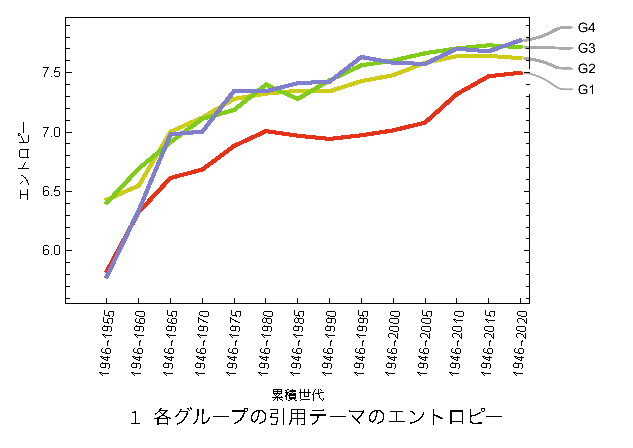
\includegraphics[width=55mm]{entropymesh-1.eps} & 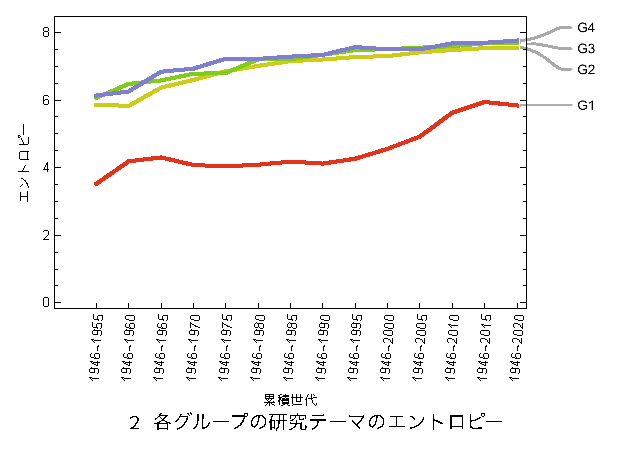
\includegraphics[width=55mm]{entropymesh-2.eps} & 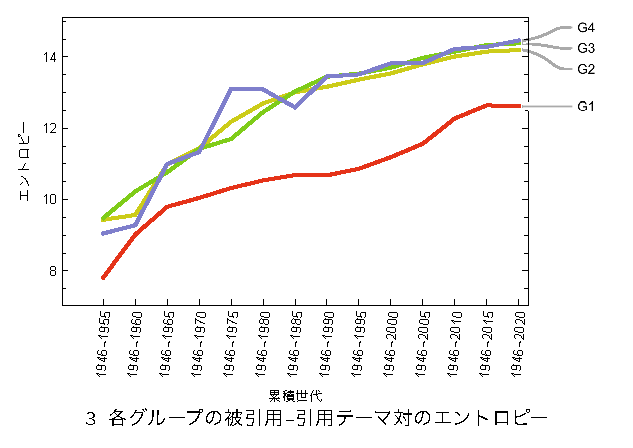
\includegraphics[width=55mm]{entropymesh-3.eps} \\
  \end{tabular}
  }
  \caption{累積世代、論文グループごとの研究テーマの出現に関するエントロピー}
  \label{fig:arr2}
\end{center}
\end{figure*}

\begin{figure}[h]
\begin{center}
  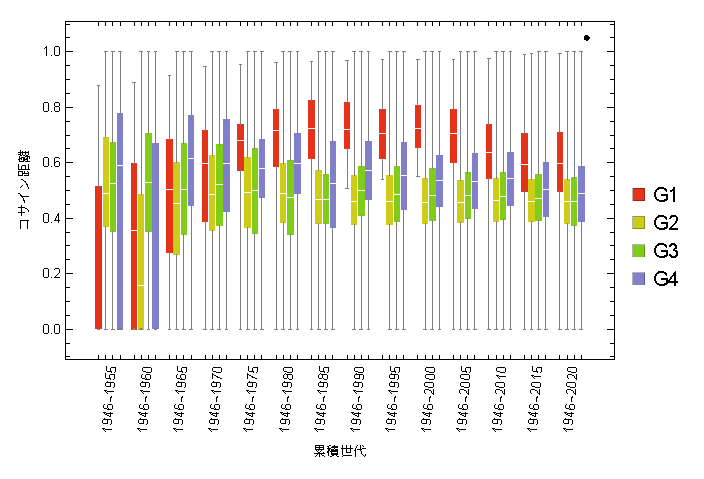
\includegraphics[width=76mm]{meshpivotatGen.eps}
  \caption{累積世代、論文グループごとの被引用テーマに対する引用テーマの転換の程度}
  \label{fig:meshpivot}
\end{center}
\end{figure}

\begin{figure}[h]
\begin{center}
  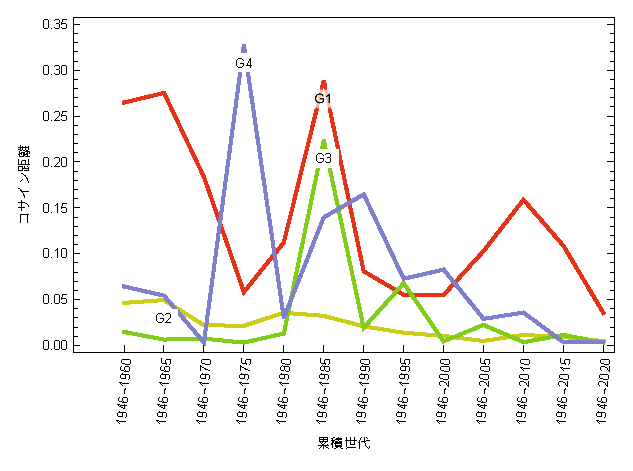
\includegraphics[width=76mm]{gr15.eps}
  \caption{論文グループごとの累積世代間の研究テーマの転換の程度}
  \label{fig:gr15}
\end{center}
\end{figure}


\section{まとめ}
高被引用論文のオブソレッセンス：
高被引用論文はその被引用の累積的な効果により長期にわたり上位の順位を維持するものの、最終的には減衰が確認され、新しい累積世代の論文にその座を明け渡す現象を確認できた。この交代までの期間は非常に長く最長で50年以上であった。うち、オブソレッセンスが確認された論文集合では、既存の報告と比べ、ピーク年（出版後に最大被引用数に達する年）が長くなる傾向があり、これは高被引用論文でのみ見られた。

高被引用論文掲載誌の特徴：
高被引用論文が必ずしもトップクラスの高インパクトファクター誌に掲載されるわけではないことが明らかになった。つまり、実際にはよりインパクトファクターの高い雑誌が収録されているにもかかわらず、高被引用論文掲載誌においてそのような雑誌の出現を確認できなかった。
とはいえ、高被引用論文掲載誌には、他のグループに比べインパクトファクターが高い雑誌も見られた。
高被引用論文の雑誌への嗜好については、特定の雑誌の確認はできなかったが、KLDによる分析から他のグループに比べより集中的であることが明らかになった。

高被引用テーマと高被引用論文引用テーマ：
高被引用論文は、研究テーマは集中的であるが、異なるテーマの論文から引用されやすいことが明らかになった。高被引用論文は、研究テーマおよび引用テーマそれぞれを個別に見た場合の多様性は低いが、研究テーマ対引用テーマの転換という観点では転換の程度が高くなる。もしこれがオブソレッセンスに影響しているのだとすれば、様々な研究領域から興味を持たれるようなテーマの論文は長く引用され続けるのかもしれない。前述の雑誌の特徴に照らせば、高被引用論文掲載誌に、幅広い領域から興味を持たれるであろう基礎領域や学際的分野の雑誌が見られる一方で、医学や医工学といった特定の応用領域の雑誌が見られないことも、これを示唆している。

長期的な傾向：
本研究ではさまざまな指標を用いたが、経年的な傾向が見られたものは少なかった。
唯一、引用テーマ/被引用テーマ/引用テーマ-被引用テーマ対のエントロピーに上昇傾向が見られた。

累積的な被引用データの影響：
累積の影響期間を変動させた順位相関の分析の結果、累積的な被引用を用いることにより順位の変動が大きくなった。すなわち累積的な被引用データを用いることは、順位等の相対的な評価のダイナミクスを上昇させることにつながる。


%\FloatBarrier
%\balance
\bibliographystyle{ujsik}
\bibliography{ama.utf8}

\end{document}
